
\begin{figure}[htbp]
\centering
\includegraphics[height=8cm]{figures/Photodiodebox.pdf}
\includegraphics[height=8cm]{figures/Photodiodebox2.pdf}
\caption{View of the Photodiode box}\label{fig:lasphotodiodebox}
\end{figure}

The photodiode box is a 3U subrack kit (Europac Pro 3U-84F P236 24563172 from Schroff) adapted to contain (figure \ref{fig:lasphotodiodebox}):
\begin{itemize}
\item a set of ten modules dubbed cassettes; each cassette incorporates a Si PIN photodiode (Hamamatsu S3590-08) coupled to a preamplifier (see figure xx). The photodiode is equipped with an epoxy resin window, has an active area of 10x10 mm and a peak sensitivity wavelength of 960 nm. A reverse voltage of 12 V is applied.
\item LicPhD card (Fig. \ref{fig:laslicphd}) : this module provides measurements of  the temperature and the humidity inside the K7. It is also used to set the polarization of the photodiodes and to
manage the interlock chain that prevents users from flashing the \laser~when the optics box is open.

\begin{figure}[htbp]
\centering
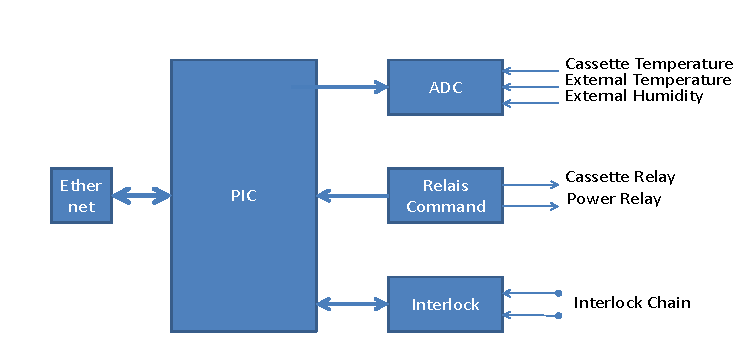
\includegraphics[height=4cm]{figures/licphd_scheme.pdf}
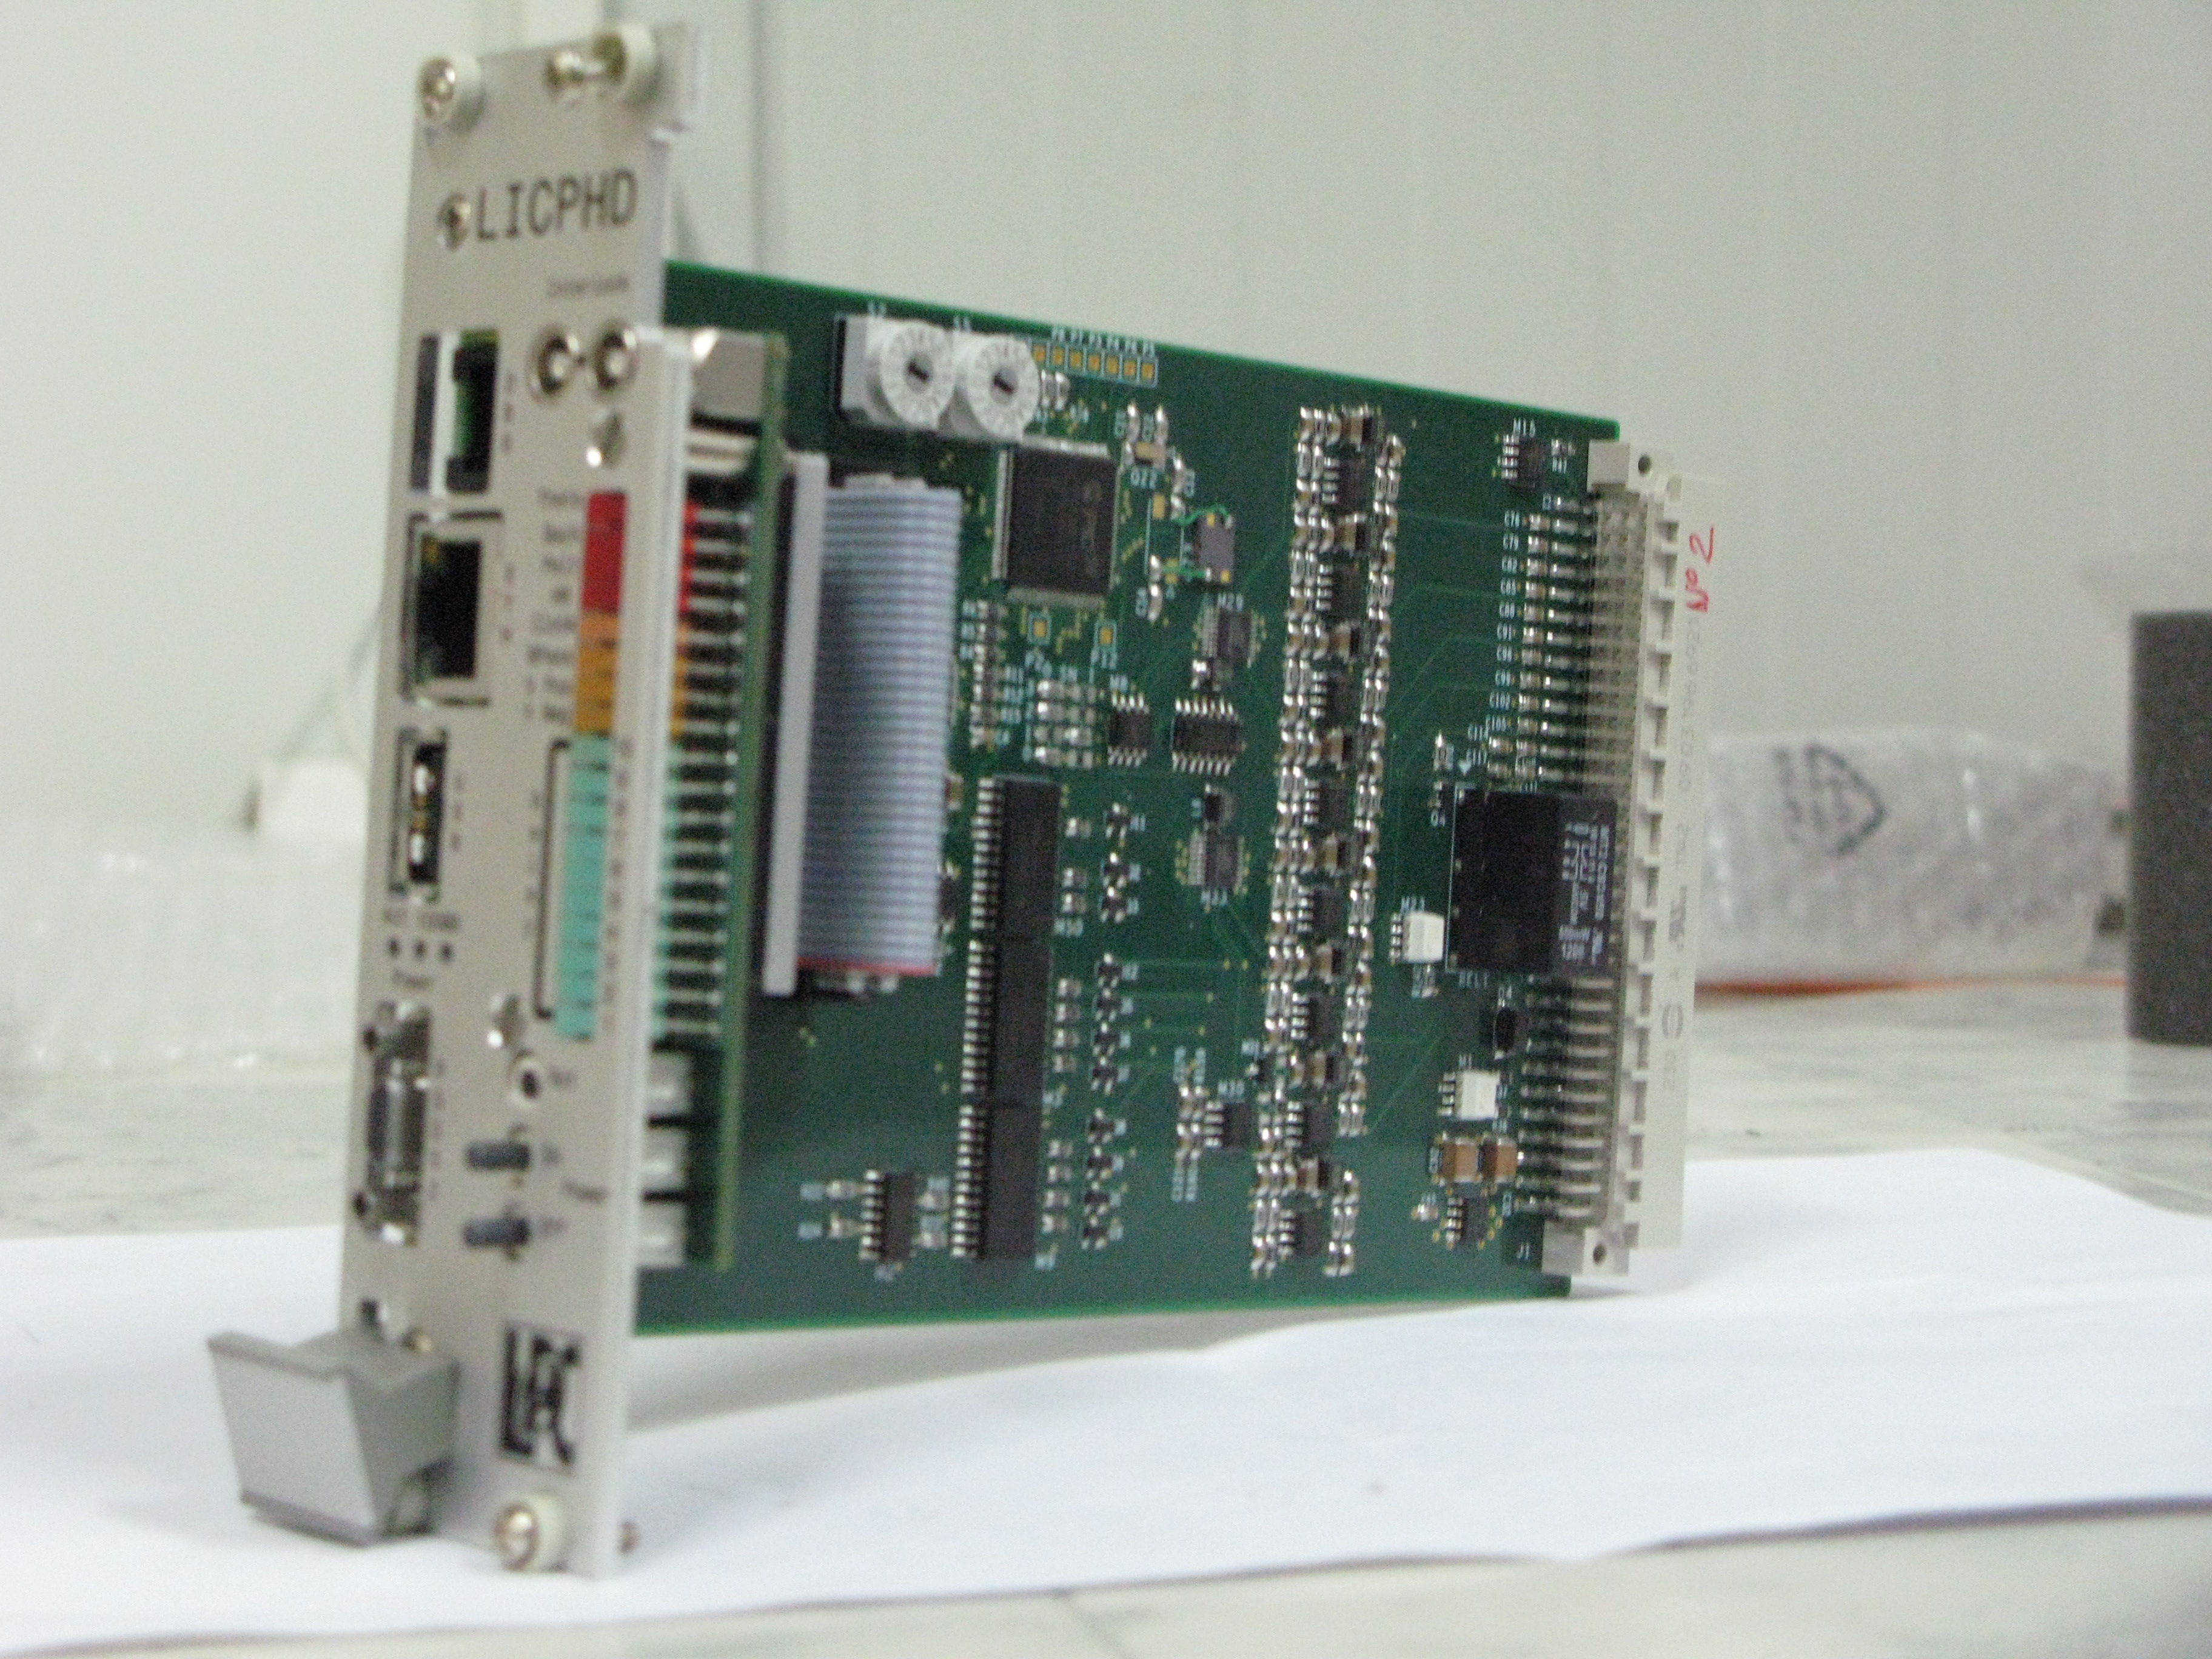
\includegraphics[height=4cm]{figures/licphd.JPG}
\caption{View of the LicPhD card}\label{fig:laslicphd}
\end{figure}

\item \charinjsplit~card

The \charinjsplit~card (Fig. \ref{fig:lascis}) transmits the charge issued by the LILAS card (lemo connector) to the preamplifiers inside the cassettes (special connector at the rear of the photodiode box). 
\begin{figure}[htbp]
\centering
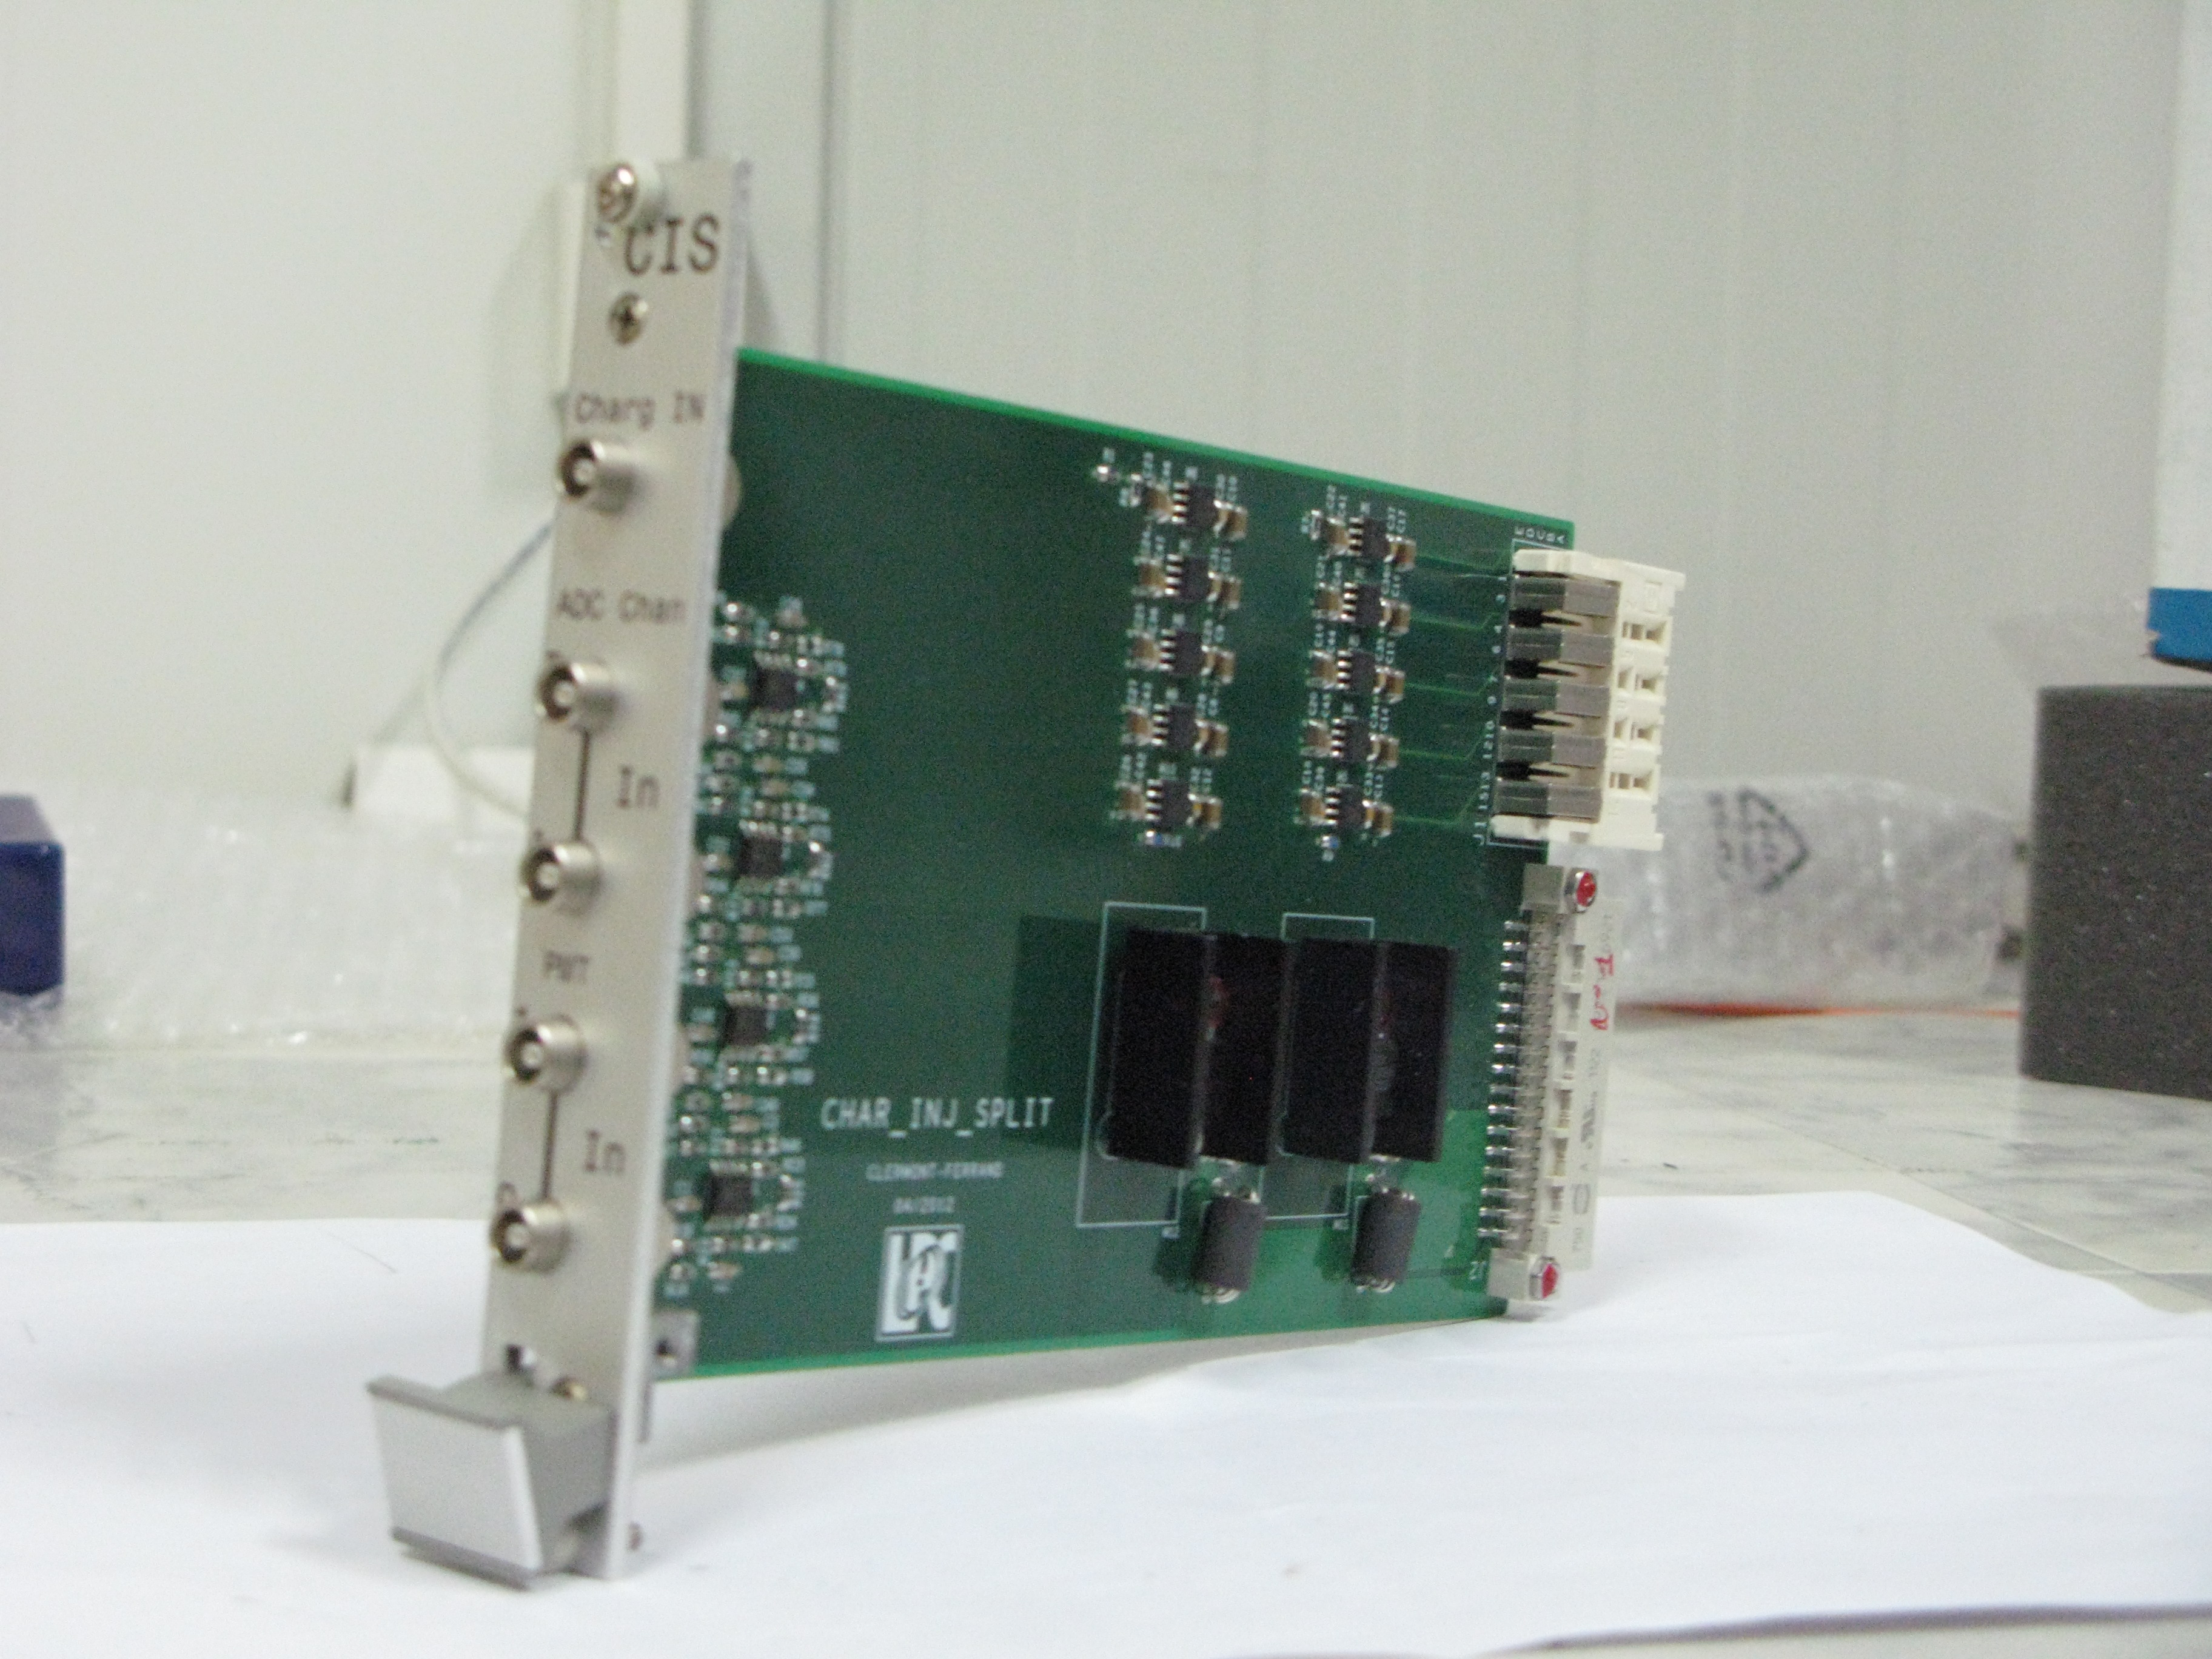
\includegraphics[height=5cm]{figures/cis.JPG}
\caption{View of the  \charinjsplit~card}\label{fig:lascis}
\end{figure}

\item Optic fibers: a set of two optics fibers is conncected at the rear end of the photodiode box, in front of each photodiode. One of this fiber is connected to the rear of phocal and is used to transmit the light emitted by the LED. The other fiber conveys the \laser~light and is plugged to the patch panel of optical filters. 
\item Deflectors
In USA15, electronics is cooled thanks to an air flow circulating from the bottom to the top of the racks. This flux may stir optics fibers plugged at the rear of the photodiode box, inducing a change of the curvature radius and hence a variation of the amount of light transmitted. Deflectors have been designed to minimize this effect and to ensure a stable configuration (in terms of position and curvature radius) of the optics fibers.
\end{itemize}


